\documentclass[article]{jss}

%% -- LaTeX packages and custom commands ---------------------------------------

%% recommended packages
\usepackage{orcidlink,lmodern,amsmath}

%% another package (only for this demo article)
\usepackage{framed}

%% new custom commands
\newcommand{\class}[1]{`\code{#1}'}
\newcommand{\fct}[1]{\code{#1()}}


%% -- Article metainformation (author, title, ...) -----------------------------

%% - \author{} with primary affiliation (and optionally ORCID link)
%% - \Plainauthor{} without affiliations
%% - Separate authors by \And or \AND (in \author) or by comma (in \Plainauthor).
%% - \AND starts a new line, \And does not.
\author{Selçuk Korkmaz~\orcidlink{0000-0003-4632-6850}\\Trakya University}
\Plainauthor{Selçuk Korkmaz}

%% - \title{} in title case
%% - \Plaintitle{} without LaTeX markup (if any)
%% - \Shorttitle{} with LaTeX markup (if any), used as running title
\title{bioLeak: Leakage-Aware Modeling and Diagnostics for Machine Learning in \proglang{R}}
\Plaintitle{bioLeak: Leakage-Aware Modeling and Diagnostics for Machine Learning in R}
\Shorttitle{Leakage-Aware Modeling in \proglang{R}}

%% - \Abstract{} almost as usual
\Abstract{
Data leakage remains a recurrent source of optimistic bias in biomedical machine
learning studies. Standard row-wise cross-validation and globally estimated
preprocessing steps are often inappropriate for data with repeated
measurements, study-level heterogeneity, batch effects, or temporal
dependencies. This paper describes \texttt{bioLeak}, an \proglang{R} package for
constructing leakage-aware resampling workflows and for auditing fitted models
for common leakage mechanisms. The package provides leakage-aware split
construction, train-fold-only preprocessing, cross-validated model fitting,
nested hyperparameter tuning, post hoc leakage audits, and HTML reporting.
Primary interfaces include \texttt{make\_split\_plan()},
\texttt{fit\_resample()}, \texttt{tune\_resample()},
\texttt{audit\_leakage()}, \texttt{audit\_report()}, and
\texttt{delta\_lsi()}. The implementation supports binary classification,
multiclass classification, and survival analysis for modeling, with
task-specific metrics and S4 containers for splits, fits, audits, and
inflation summaries. Results reported in this manuscript are drawn from stored
simulation and case-study outputs in the package paper directory rather than
from newly executed experiments. The simulation artifacts show how apparent
performance changes under controlled leakage mechanisms, and the case study
illustrates how guarded and naive pipelines can yield materially different
conclusions on multi-study transcriptomic data. The emphasis throughout is on
software design, reproducible workflows, and interpretation of diagnostic
output.
}

%% - \Keywords{} with LaTeX markup, at least one required
%% - \Plainkeywords{} without LaTeX markup (if necessary)
%% - Should be comma-separated and in sentence case.
\Keywords{biomedical machine learning, data leakage,
cross-validation, reproducibility, resampling, auditing, R, \proglang{R}}
\Plainkeywords{biomedical machine learning, data leakage, cross-validation, reproducibility, resampling, auditing, R}

%% - \Address{} of at least one author
%% - May contain multiple affiliations for each author
%%   (in extra lines, separated by \emph{and}\\).
%% - May contain multiple authors for the same affiliation
%%   (in the same first line, separated by comma).
\Address{
  Selçuk Korkmaz\\
  Department of Biostatistics and Medical Informatics\\
  Faculty of Medicine\\
  Trakya University\\
  Balkan Yerleşkesi\\
  22030 Edirne, Türkiye\\
  E-mail: \email{selcukorkmaz@gmail.com}\\
  URL: \url{https://selcukorkmaz.github.io/}
}

\begin{document}


%% -- Introduction -------------------------------------------------------------

%% - In principle "as usual".
%% - But should typically have some discussion of both _software_ and _methods_.
%% - Use \proglang{}, \pkg{}, and \code{} markup throughout the manuscript.
%% - If such markup is in (sub)section titles, a plain text version has to be
%%   added as well.
%% - All software mentioned should be properly \cite-d.
%% - All abbreviations should be introduced.
%% - Unless the expansions of abbreviations are proper names (like "Journal
%%   of Statistical Software" above) they should be in sentence case (like
%%   "generalized linear models" below).

\section[Introduction]{Introduction} \label{sec:intro}

Cross-validated performance estimates are often treated as evidence that a
predictive model will generalize to future biomedical data. That interpretation
depends on assumptions that are frequently violated in practice: observations
must be exchangeable with respect to the resampling design, preprocessing must
be estimated without access to evaluation data, and the outcome must not be
recoverable from proxy variables that are unavailable at prediction time.
Violations of these assumptions are usually described as data leakage. Leakage
is not a narrow implementation detail. It affects whether model accuracy,
feature importance, calibration, and downstream biological interpretation are
credible. This concern has been emphasized across data mining, statistical
learning, and biomedical prediction, including early discussions of selection
bias in microarray studies \citep{ambroise2002}, broader treatments of
leakage in data mining \citep{kaufman2012}, warnings about genomic prediction
pitfalls \citep{simon2003, subramanian2013}, and recent accounts
linking leakage to wider reproducibility failures in machine-learning-based
science \citep{kapoor2023}. Related evaluation biases also arise when
model selection is not nested appropriately within resampling, a point stressed
by \citet{varma2006} and \citet{cawley2010}.

The problem is especially acute in biomedical applications. A single study may
contain repeated measurements from the same participant, technical replicates,
laboratory batches, study-site effects, or longitudinal samples collected over
time. In such settings, row-wise cross-validation can place correlated samples
in both training and test folds. Similarly, global imputation, normalization,
or feature filtering performed before resampling can transmit test-fold
information into the training pipeline. These choices can inflate performance
while leaving no obvious trace in a conventional model summary, a practical
problem in health-care machine learning where evaluation, implementation, and
deployment constraints are already difficult to align \citep{beam2018, sendak2019}.

Recent methodological work has documented the scale of the issue. \citet{kapoor2023} described leakage as a contributor to broader reproducibility
failures in machine-learning-based science. \citet{rosenblatt2024} showed in
neuroimaging that feature-selection and repeated-subject leakage can
substantially inflate predictive performance, while \citet{vandemortel2025} reported that leakage-compatible practices were common enough to
affect meta-analytic conclusions in psychiatric imaging. In clinical
prediction, \citet{davis2024} discussed label leakage induced by workflow
artifacts rather than by explicit coding mistakes. These studies do not imply
that leakage can be removed by a single rule. Rather, they show that leakage is
heterogeneous, domain specific, and tightly linked to evaluation design.

Existing modeling frameworks provide much of the infrastructure needed for
modern predictive analysis, but they do not remove the need to define
appropriate leakage boundaries. In \proglang{R} \citep{R}, \texttt{caret}, \texttt{tidymodels}, and
\texttt{mlr3} support flexible resampling, preprocessing, and model-fitting
workflows \citep{kuhn2008, kuhn2020, lang2019, bischl2024}. These frameworks can be used safely, but they rely on the analyst to
specify resampling units, grouping variables, and fold-wise preprocessing
correctly. In biomedical applications, where rows are often nested within
subjects, batches, studies, or time windows, the critical difficulty is not
only fitting a model but encoding the structured dependencies that determine
which observations may legitimately share information.

\texttt{bioLeak} was developed to support two related tasks. The first is
prevention: constructing resampling and preprocessing workflows that reduce the
risk of train-test contamination. The second is diagnosis: auditing fitted
cross-validated models for evidence that apparent performance may depend on
leakage or confounding. The package therefore combines leakage-aware split
plans, guarded preprocessing, cross-validated fitting, nested tuning,
post-fitting audits, and reporting utilities in a single R workflow. The
package is designed for practical use with tabular biomedical data and
\texttt{SummarizedExperiment} objects, and it interoperates with common R
modeling infrastructure such as \texttt{parsnip}, \texttt{recipes},
\texttt{workflows}, \texttt{yardstick}, and \texttt{rsample}.

This manuscript follows the software-oriented emphasis expected for the Journal
of Statistical Software. Section~2 summarizes the leakage mechanisms that
motivate the package. Section~3 describes the main software components.
Section~4 presents a reproducible workflow based on the package API.
Section~5 defines the \texttt{Delta Leakage Sensitivity Index} framework used
to quantify inflation between naive and guarded pipelines. Sections~6 and 7
describe simulation and case-study results using stored paper artifacts.
Section~8 discusses implementation details, Section~9 reviews limitations and
future work, and Section~10 records current software availability.


%% -- Manuscript ---------------------------------------------------------------

%% - In principle "as usual" again.
%% - When using equations (e.g., {equation}, {eqnarray}, {align}, etc.
%%   avoid empty lines before and after the equation (which would signal a new
%%   paragraph.
%% - When describing longer chunks of code that are _not_ meant for execution
%%   (e.g., a function synopsis or list of arguments), the environment {Code}
%%   is recommended. Alternatively, a plain {verbatim} can also be used.
%%   (For executed code see the next section.)

\section{Data Leakage in Biomedical Machine Learning}\label{sec:leakage}
\subsection{Preprocessing leakage}

Preprocessing leakage occurs when statistics used to transform predictors are
estimated using all samples rather than only the training fold. Common examples
include global missing-value imputation, normalization, variance filtering, and
feature selection performed before resampling. \citet{moscovich2022}
showed that even unsupervised preprocessing can bias cross-validation when it
is estimated outside the resampling loop, a common failure mode in biomedical
pipelines that treat normalization and filtering as preliminary cleaning rather
than as model components. In genomics, the same concern appears as feature-
selection bias: selecting genes before resampling can produce highly optimistic
error estimates even when the downstream classifier is simple \citep{ambroise2002, simon2003, subramanian2013}.

\subsection{Dependent samples and subject overlap}

Many biomedical datasets contain repeated measures, multi-region samples from
the same patient, family-related observations, or longitudinal observations
from the same person. If row-wise resampling is applied, records from the same
latent unit can appear in both training and test folds. In that case the model
may recognize subject identity rather than the biological signal of interest.
This problem is especially acute when outcomes are stable within subject or
when repeated measurements are dense. More generally, the problem belongs to
the broader class of structured-resampling failures discussed by \citet{roberts2017}, \citet{wenger2012}, and \citet{valavi2019}, where naive row-wise
fold assignment ignores dependencies induced by space, time, hierarchy, or
shared latent units.

\subsection{Batch and study confounding}

High-throughput molecular assays frequently exhibit batch effects associated
with laboratory, plate, scanner, platform, or study site. If outcome labels are
unevenly distributed across these technical groups, a model can use batch as a
surrogate for outcome. \citet{soneson2014} and \citet{hamdan2023} showed
that such confounding, and even attempted confound removal, can distort
cross-validation-based estimates. In a multi-study setting, however, the
intended validation target matters: if one study is held out at a time for
external validation, perfect fold-study association is expected and should not
be interpreted as a software error. This is one instance of the more general
principle that resampling must respect the dependence structure relevant to the
intended deployment target \citep{roberts2017}.

\subsection{Temporal look-ahead leakage}

When data have a temporal order, a random split permits the training set to use
information that would not have been available at the prediction time of the
test set. The most direct example is an explicit future variable, such as a
subsequent laboratory measurement or a later event summary, included as a
predictor. A subtler example arises when preprocessing borrows strength across
future observations. Proper time-aware resampling therefore requires
chronological ordering and, in some settings, purge or embargo windows to
prevent overlap between training and evaluation periods. The same point appears
in broader cross-validation methodology: evaluation is meaningful only when the
data split matches the prediction task that the model is meant to serve \citep{stone1974, arlot2010, hastie2009}.

\subsection{Target leakage and duplicate samples}

Target leakage occurs when a predictor carries direct information about the
outcome definition. In electronic health records this may be a billing code or
medication that is downstream of the diagnosis. In multi-omics or public
expression resources it may be a transformed outcome summary or a feature
engineered using labels. Duplicate and near-duplicate samples are related but
distinct: they need not encode the outcome explicitly, yet a nearly identical
training sample can make a test sample artificially easy to predict. Because
such problems may survive apparently careful resampling, they are a natural
target for post hoc diagnostics. In audit terms, near-duplicate detection is
closer to record linkage or similarity search than to classical hypothesis
testing, and it inherits familiar design choices about feature representation,
matching rules, and thresholds \citep{winkler1999, christen2012, leskovec2014}.

\section[Overview of the bioLeak Package]{Overview of the \texttt{bioLeak} Package}

The package is organized around four design goals: leakage-aware modeling,
reproducible workflows, diagnostic auditing, and compatibility with common R
modeling tools. The software focuses on biomedical prediction studies in which
the user already has a labeled dataset and wants to evaluate whether reported
performance may depend on leakage or confounding.

Figure~\ref{fig:workflow} summarizes the main package workflow from a labeled
dataset to fitted resampling results, audit summaries, and inflation
quantification.

\begin{figure}[tbp]
\centering
\fbox{\parbox{0.38\linewidth}{\centering
Dataset \\
$\downarrow$ \\
\texttt{make\_split\_plan()} \\
$\downarrow$ \\
\textit{SplitPlan} \\
$\downarrow$ \\
\texttt{fit\_resample()} \\
$\downarrow$ \\
\textit{ResampleFit} \\
$\downarrow$ \\
\texttt{audit\_leakage()} \\
$\downarrow$ \\
\textit{LeakAudit} \\
$\downarrow$ \\
\texttt{delta\_lsi()} \\
$\downarrow$ \\
\textit{LeakDeltaLSI}}}
\caption{\texttt{bioLeak} leakage-aware modeling workflow. The conceptual
stages shown in the diagram correspond to the implemented S4 objects described
in the main text.}
\label{fig:workflow}
\end{figure}

In the implemented API, these conceptual stages correspond to the S4 classes
\texttt{LeakSplits}, \texttt{LeakFit}, \texttt{LeakAudit}, and
\texttt{LeakDeltaLSI}. The conceptual names are useful for exposition, while
the class names are the objects users encounter in code and printed summaries.

The main workflow begins with \texttt{make\_split\_plan()}, which constructs an
S4 \texttt{LeakSplits} object. The split plan records the resampling mode,
fold-level indices or compact fold assignments, and metadata such as the
grouping variables, number of folds, number of repeats, and a reproducibility
hash. The split modes most relevant to the present manuscript are
\texttt{subject\_grouped}, \texttt{batch\_blocked},
\texttt{study\_loocv}, and \texttt{time\_series}. These modes address distinct
dependence structures rather than acting as interchangeable cross-validation
variants.

Model fitting is handled by \texttt{fit\_resample()}, which applies guarded
preprocessing independently within each fold, trains one or more learners, and
returns a \texttt{LeakFit} object. The fit object stores per-fold metrics,
aggregated summaries, audit metadata, predictions, preprocessing state,
learners, and information required for later refit-based audits. The function
accepts data frames, matrices, and \texttt{SummarizedExperiment} objects.
Learners may be specified through \texttt{parsnip}, \texttt{workflows}, legacy
character interfaces, or custom fit/predict pairs.

\texttt{tune\_resample()} extends this design to nested resampling. Outer folds
are defined by a \texttt{LeakSplits} object or an \texttt{rsample} structure
that already contains inner folds. Tuning results are returned as a
\texttt{LeakTune} object containing inner tuning outputs, outer-fold metrics,
selected hyperparameters, optional threshold selections for binary outcomes, and
an optional refitted final workflow. Survival tasks are currently excluded from
\texttt{tune\_resample()}.

Auditing is provided by \texttt{audit\_leakage()}, which returns a
\texttt{LeakAudit} object. The audit combines a permutation-gap analysis, fold
association tests for batch or study metadata, target-leakage scans on a
reference feature matrix, duplicate detection, and a compact mechanism-level
summary stored in the object metadata. \texttt{audit\_report()} renders these
results to a self-contained HTML report based on a bundled R Markdown template.
For direct inflation comparisons between a naive and a guarded pipeline, the
package also provides \texttt{delta\_lsi()}, which returns a
\texttt{LeakDeltaLSI} object summarizing repeat-level performance differences,
robust point estimates, confidence intervals, and sign-flip randomization
tests.

Table~\ref{tab:components} lists the primary user-facing functions and their
roles in the workflow.

\begin{table}[tbp]
\centering
\caption{Primary software components in \texttt{bioLeak}.}
\label{tab:components}
\begin{tabular}{|p{0.21\linewidth}|p{0.25\linewidth}|p{0.42\linewidth}|}
\hline
\textbf{Stage} & \textbf{Primary function(s)} & \textbf{Main output or role} \\
\hline
Split construction & \texttt{make\_split\_plan()} & Leakage-aware split plans for subject, batch, study, or time-ordered resampling. \\
\hline
Cross-validated fitting & \texttt{fit\_resample()} & Fold predictions, fold metrics, aggregated performance summaries, preprocessing state, and refit metadata. \\
\hline
Nested tuning & \texttt{tune\_resample()} & Nested cross-validation for hyperparameter tuning with leakage-aware outer and inner folds. \\
\hline
Leakage auditing & \texttt{audit\_leakage()} & Permutation-gap summaries, batch or study association tests, target scans, duplicate detection, and mechanism summaries. \\
\hline
Audit reporting & \texttt{audit\_report()} & Self-contained HTML summaries suitable for review and supplementary material. \\
\hline
Inflation quantification & \texttt{delta\_lsi()} & Repeat-level comparison of naive and guarded pipelines, including robust inflation estimates and randomization-based inference. \\
\hline
Interoperability & \texttt{guard\_to\_recipe()}, \texttt{as\_rsample()} & Bridges to \texttt{recipes} and \texttt{rsample} workflows. \\
\hline
\end{tabular}
\end{table}

\section{Leakage-Aware Modeling Workflow}

This section illustrates a typical workflow using a small synthetic binary
classification example. The same workflow structure extends to multiclass and
survival tasks, although the available metrics and some audit components differ.
The underlying evaluation logic follows standard resampling principles, but it
adapts them to structured biomedical data in which the independence unit may be
subject, batch, study, or time rather than row \citep{stone1974, kohavi1995, arlot2010, james2013}.

\subsection{Constructing a split plan}

The first step is to define the dependence structure that the resampling design
should respect. In the example below, repeated measurements are nested within
subject, so a subject-grouped split plan is used. The code mirrors the current
package API and can be adapted to \texttt{batch\_blocked},
\texttt{study\_loocv}, or \texttt{time\_series} by replacing the relevant mode
and metadata columns.

\begin{verbatim}
library(bioLeak)
library(parsnip)

set.seed(1)
n_subject <- 40
rep_per_subject <- 3
n <- n_subject * rep_per_subject

subject <- rep(seq_len(n_subject), each = rep_per_subject)
batch <- rep(seq_len(6), length.out = n)
x1 <- rnorm(n)
x2 <- rnorm(n)
x3 <- rnorm(n)
subject_signal <- rnorm(n_subject)
outcome <- factor(
  ifelse(runif(n) < plogis(subject_signal[subject]), "case", "control"),
  levels = c("control", "case")
)

df <- data.frame(subject, batch, outcome, x1, x2, x3)

splits <- make_split_plan(
  df,
  outcome = "outcome",
  mode = "subject_grouped",
  group = "subject",
  v = 5,
  stratify = TRUE,
  seed = 1
)
\end{verbatim}

\noindent
The split object records fold membership and split metadata. For large
datasets, \texttt{compact = TRUE} stores fold assignments rather than explicit
index lists to reduce memory use.

\subsection{Defining guarded preprocessing}

\texttt{fit\_resample()} accepts either a native guarded preprocessing
specification or a \texttt{recipes::recipe}. The native interface applies each
step on the training fold only and transfers the resulting parameters to the
test fold. Supported operations include winsorization, imputation,
normalization, filtering, and feature selection. In the example below, median
imputation and z-score normalization are performed within each training fold.

\begin{verbatim}
spec <- logistic_reg(mode = "classification") |>
  set_engine("glm")

fit_guarded <- fit_resample(
  df,
  outcome = "outcome",
  splits = splits,
  learner = spec,
  metrics = "auc",
  preprocess = list(
    impute = list(method = "median"),
    normalize = list(method = "zscore"),
    filter = list(var_thresh = 0, iqr_thresh = 0),
    fs = list(method = "none")
  ),
  refit = FALSE,
  seed = 1
)
\end{verbatim}

\noindent
For multiclass classification, the same interface can be used with metrics such
as \texttt{accuracy}, \texttt{macro\_f1}, and \texttt{log\_loss}. For survival
analysis, the outcome is specified as a two-element character vector containing
time and event columns, and the principal metric is the concordance index.

\subsection{Training naive and guarded comparators}

The package is most informative when a guarded analysis is accompanied by a
plausible naive or intentionally leaky comparator. The next snippet adds a
subject-level leakage proxy and fits an otherwise identical pipeline. Such
comparisons are useful both for exploratory sensitivity analysis and for the
\texttt{delta\_lsi()} procedure described in Section~5.

\begin{verbatim}
df_leaky <- within(df, {
  leak_subject <- ave(as.numeric(outcome == "case"), subject, FUN = mean)
})

fit_naive <- fit_resample(
  df_leaky,
  outcome = "outcome",
  splits = splits,
  learner = spec,
  metrics = "auc",
  preprocess = list(
    impute = list(method = "none"),
    normalize = list(method = "none"),
    filter = list(var_thresh = 0, iqr_thresh = 0),
    fs = list(method = "none")
  ),
  refit = FALSE,
  seed = 1
)
\end{verbatim}

\subsection{Auditing a fitted workflow}

After cross-validated predictions have been generated, \texttt{audit\_leakage()}
can be used to summarize the evidence available within the fitted object and,
optionally, in an aligned reference matrix \texttt{X\_ref}. The reference
matrix enables target-leakage scans and duplicate detection. In grouped designs,
the same audit interface can be used with restricted permutations and
batch-association tests.

\begin{verbatim}
audit_guarded <- audit_leakage(
  fit_guarded,
  metric = "auc",
  B = 50,
  perm_stratify = TRUE,
  X_ref = df[, c("x1", "x2", "x3")],
  batch_cols = "batch",
  return_perm = TRUE
)

summary(audit_guarded)
\end{verbatim}

\noindent
The resulting \texttt{LeakAudit} object stores one-row permutation summaries,
feature-level target-association results, duplicate pairs, and a trail of audit
parameters. The permutation module is diagnostic rather than dispositive: a
large positive gap indicates non-random predictive signal, but the other audit
components are needed to assess whether that signal may be inflated by leakage.

\subsection{Generating an HTML audit report}

The audit can be rendered into an HTML report without modifying the underlying
fit object. The report is particularly useful when a model review requires a
human-readable appendix.

\begin{verbatim}
report_file <- audit_report(
  audit_guarded,
  output_file = "bioLeak_audit_report.html",
  output_dir = tempdir(),
  quiet = TRUE
)
\end{verbatim}

\subsection{Putting the workflow together}

The previous subsections present each stage separately. In practice, the full
workflow is usually executed as one analysis script that constructs a split
plan, fits guarded and naive comparators, audits the guarded fit, quantifies
inflation, and renders a report. The following code block illustrates that
sequence in one place.

\begin{verbatim}
library(bioLeak)
library(parsnip)

set.seed(1)
n_subject <- 30
rep_per_subject <- 4
n <- n_subject * rep_per_subject

subject <- rep(seq_len(n_subject), each = rep_per_subject)
batch <- rep(seq_len(6), length.out = n)
latent <- rnorm(n_subject)
x1 <- latent[subject] + rnorm(n, sd = 0.5)
x2 <- rnorm(n)
x3 <- rnorm(n)
outcome <- factor(
  ifelse(runif(n) < plogis(latent[subject]), "case", "control"),
  levels = c("control", "case")
)

dat <- data.frame(subject, batch, outcome, x1, x2, x3)

plan <- make_split_plan(
  dat,
  outcome = "outcome",
  mode = "subject_grouped",
  group = "subject",
  v = 5,
  stratify = TRUE,
  seed = 1
)

spec <- logistic_reg(mode = "classification") |>
  set_engine("glm")

fit_guarded <- fit_resample(
  dat,
  outcome = "outcome",
  splits = plan,
  learner = spec,
  metrics = "auc",
  preprocess = list(
    impute = list(method = "median"),
    normalize = list(method = "zscore"),
    filter = list(var_thresh = 0, iqr_thresh = 0),
    fs = list(method = "none")
  ),
  refit = FALSE,
  seed = 1
)

dat_naive <- within(dat, {
  leak_subject <- ave(as.numeric(outcome == "case"), subject, FUN = mean)
})

fit_naive <- fit_resample(
  dat_naive,
  outcome = "outcome",
  splits = plan,
  learner = spec,
  metrics = "auc",
  preprocess = list(
    impute = list(method = "none"),
    normalize = list(method = "none"),
    filter = list(var_thresh = 0, iqr_thresh = 0),
    fs = list(method = "none")
  ),
  refit = FALSE,
  seed = 1
)

audit <- audit_leakage(
  fit_guarded,
  metric = "auc",
  B = 50,
  perm_stratify = TRUE,
  batch_cols = "batch",
  X_ref = dat[, c("x1", "x2", "x3")]
)

delta <- delta_lsi(
  fit_naive = fit_naive,
  fit_guarded = fit_guarded,
  metric = "auc",
  seed = 1
)

report_file <- audit_report(
  audit,
  output_file = "bioLeak_audit_report.html",
  output_dir = tempdir(),
  quiet = TRUE
)
\end{verbatim}

\noindent
The split plan defines the dependence structure, \texttt{fit\_resample()}
trains the guarded and naive pipelines under that design, \texttt{audit} stores
diagnostic evidence for the guarded fit, \texttt{delta} summarizes the
repeat-level inflation between the naive and guarded analyses, and
\texttt{audit\_report()} produces a shareable HTML summary. The same pattern
extends to multiclass and survival settings with task-appropriate learners and
metrics.

\subsection{Leakage-safe hyperparameter tuning}

\texttt{tune\_resample()} performs nested cross-validation so that model
selection remains inside the outer resampling loop. The example below uses a
tunable \texttt{glmnet} specification and an inner resampling structure derived
from a nested split plan. This design avoids tuning on the same assessment data
used for outer-loop evaluation.

\begin{verbatim}
library(recipes)
library(tune)

nested_splits <- make_split_plan(
  df,
  outcome = "outcome",
  mode = "subject_grouped",
  group = "subject",
  v = 3,
  nested = TRUE,
  seed = 14
)

rec <- recipe(outcome ~ x1 + x2 + x3, data = df) |>
  step_impute_median(all_numeric_predictors()) |>
  step_normalize(all_numeric_predictors())

spec_tune <- logistic_reg(
  penalty = tune(),
  mixture = 1,
  mode = "classification"
) |>
  set_engine("glmnet")

tuned <- tune_resample(
  df,
  outcome = "outcome",
  splits = nested_splits,
  learner = spec_tune,
  preprocess = rec,
  grid = 5,
  metrics = c("auc", "accuracy"),
  selection = "one_std_err",
  refit = TRUE,
  seed = 14
)
\end{verbatim}

\noindent
When a \texttt{recipe} or \texttt{workflow} is used, \texttt{bioLeak} checks
the graph for operations that may violate fold-wise estimation rules. The
package also provides \texttt{guard\_to\_recipe()} when a guarded preprocessing
specification needs to be translated into an approximate \texttt{recipes}
pipeline.

\subsection{Practical workflow variants}

The same structure generalizes to the other supported split modes. With
\texttt{batch\_blocked}, all records from the same batch are isolated in one
fold. With \texttt{study\_loocv}, one study is held out at a time, which is
often appropriate for consortium data or data aggregated from public resources.
With \texttt{time\_series}, observations are ordered by time and training is
restricted to records that precede the test block, optionally with a prediction
horizon, purge, or embargo window. In all cases, the core principle remains the
same: resampling should represent the target deployment setting rather than a
convenient random partition of rows.

\section[Quantifying Leakage Inflation (Delta LSI)]{Quantifying Leakage Inflation (\texttt{Delta LSI})}

\texttt{bioLeak} provides \texttt{delta\_lsi()} to compare a naive pipeline
with a guarded one when both are fitted on the same repeated resampling design.
The goal is not to decide whether one pipeline is ``better'' in a generic
sense, but to quantify how much apparent performance changes when leakage
controls are introduced. This focus is consistent with the broader
cross-validation literature, which emphasizes that resampling estimates are
themselves random quantities and that their uncertainty is nontrivial to
characterize \citep{bengio2004, bates2024}.

Suppose repeated cross-validation yields $R$ repeat-level summaries. Let
$M_{\mathrm{naive},r}$ and $M_{\mathrm{guarded},r}$ denote the repeat-level
performance estimates for repeat $r$. For higher-is-better metrics such as AUC
or accuracy, the repeat-level inflation score is
\[
\Delta_r = M_{\mathrm{naive},r} - M_{\mathrm{guarded},r}, \qquad r = 1, \ldots, R.
\]
Positive values therefore indicate that the naive pipeline appears more
optimistic than the guarded one and, under the paired design, are interpreted
as leakage-related performance inflation. For lower-is-better metrics such as
RMSE or log-loss, \texttt{delta\_lsi()} applies a sign flip internally through
the \texttt{higher\_is\_better} argument so that positive values still denote
inflation.

In the implementation, fold-level metric values are aggregated to a repeat
level using test-set-size weights. Let $\mu_r$ denote the resulting repeat
summary for one pipeline. The vector
$\boldsymbol{\Delta} = (\Delta_1, \ldots, \Delta_R)^\top$ is then summarized in
two ways. The first is the arithmetic mean,
\[
\widehat{\Delta}_{\mathrm{metric}} =
\frac{1}{R} \sum_{r=1}^{R} \Delta_r,
\]
which is easy to interpret directly in the units of the metric. The second is
the robust summary reported as \texttt{delta\_lsi},
\[
\widehat{\Delta}_{\mathrm{LSI}} =
\operatorname*{arg\,min}_{\mu} \sum_{r=1}^{R}
\rho_{1.345} \left( \frac{\Delta_r - \mu}{\widehat{\sigma}} \right),
\]
where $\rho_{1.345}$ is Huber's loss function and
$\widehat{\sigma} = 1.4826 \times \mathrm{MAD}(\boldsymbol{\Delta})$ is a fixed
robust scale estimate. The Huber estimator downweights outlying repeats, which
is useful when one or two resampling repeats are unstable for reasons unrelated
to systematic leakage \citep{huber1964, huber2009}.

Confidence intervals are computed with a bias-corrected and accelerated (BCa)
bootstrap when the effective number of paired repeats is at least ten. The
package reports a $95\%$ interval for both \texttt{delta\_lsi} and the
arithmetic mean. Hypothesis testing is based on a sign-flip randomization test.
Under the null hypothesis of no systematic inflation, the sign of each
$\Delta_r$ is exchangeable. For $R \leq 15$, the package enumerates all
$2^R$ sign combinations exactly. For larger $R$, Monte Carlo sign-flips are
sampled and the Phipson-Smyth correction is applied so that the reported
$p$-value is never zero. When \texttt{exchangeability = "blocked\_time"}, a
block sign-flip procedure is used instead of the independent sign-flip test.
In this sense, the reported significance summary is a permutation-style
randomization test on the repeat-level differences rather than a model-based
large-sample approximation. The use of bootstrap intervals follows standard
resampling-based inference ideas \citep{efron1979, efron1993}.

The design is only fully inferential when the two compared fits are paired. In
practice this means they must share the same fold structure, not merely the
same number of repeats. If fold membership differs, the package falls back to an
unpaired comparison of repeat-level summaries and suppresses formal inference.
This distinction is important. If the user changes both the predictors and the
resampling design, the resulting performance difference cannot be attributed
only to leakage-aware preprocessing.

The returned \texttt{LeakDeltaLSI} object stores the metric name, the
exchangeability assumption, the effective number of paired repeats, robust and
arithmetic point estimates, bootstrap intervals, the sign-flip $p$-value, fold-
and repeat-level summaries for both pipelines, and an \texttt{info} slot with
pairing diagnostics and optional details. The package groups inferential output
into four tiers:
\begin{enumerate}
\item \texttt{D\_insufficient}: fewer than five effective paired repeats or an
unpaired comparison; point estimates only.
\item \texttt{C\_signflip}: at least five paired repeats; point estimates and a
sign-flip $p$-value.
\item \texttt{B\_signflip\_ci}: at least ten paired repeats; point estimates,
$p$-value, and BCa intervals.
\item \texttt{A\_full\_inference}: at least twenty paired repeats with finite
intervals and $p$-value.
\end{enumerate}

A typical call compares a naive and a guarded fit built from the same
\texttt{LeakSplits} object:

\begin{verbatim}
inflation <- delta_lsi(
  fit_naive = fit_naive,
  fit_guarded = fit_guarded,
  metric = "auc",
  M_boot = 2000,
  M_flip = 10000,
  seed = 42
)

summary(inflation)
\end{verbatim}

\noindent
In practice, \texttt{delta\_lsi()} is most useful when an analyst wants to
measure the sensitivity of a result to specific leakage controls, such as
subject grouping, batch blocking, or removal of explicit leak-prone features.
The case study in Section~7 demonstrates a paired comparison, and
Appendix~\ref{app:delta-lsi-sim} reports a small simulation evaluating the
Type~I error and power of the sign-flip test.

\section{Simulation Study}

\subsection{Design}

The paper repository contains a dedicated simulation script,
\texttt{paper/run\_simulation.R}, whose design is intentionally distinct from
the package-level helper \texttt{simulate\_leakage\_suite()}. The manuscript
results therefore describe the stored paper artifacts rather than package
defaults. The main result object, \texttt{paper/sim\_results\_all.rds},
contains 3{,}600 rows corresponding to a full factorial design with
\begin{itemize}
\item five leakage settings:
\texttt{none}, \texttt{subject\_overlap}, \texttt{batch\_confounded},
\texttt{peek\_norm}, and \texttt{lookahead};
\item four sample sizes: $n \in \{100, 250, 500, 1000\}$;
\item three feature dimensions: $p \in \{10, 50, 100\}$;
\item three signal levels: $s \in \{0, 0.5, 2.0\}$; and
\item twenty seeds per configuration.
\end{itemize}

For each simulated dataset, predictors were generated as Gaussian variables and
the binary outcome was sampled from a probit link applied to a latent linear
predictor. When $s = 0$, the outcome was pure noise and served as a type-I
error baseline. When $s > 0$, signal entered through the first few predictors,
and autoregressive noise was added to the latent process. Leakage was injected
as follows.
\begin{itemize}
\item \texttt{subject\_overlap}: a subject-level mean of the binary outcome was
added as a predictor.
\item \texttt{batch\_confounded}: batch membership was made outcome dependent
and the batch-wise mean outcome was added as a predictor.
\item \texttt{peek\_norm}: a noisy continuous version of the outcome was added
as a globally computed feature.
\item \texttt{lookahead}: a future biomarker value was shifted into the current
row.
\end{itemize}

All main-simulation analyses used five-fold subject-grouped cross-validation
with \texttt{glmnet} as the learner, median imputation, z-score normalization,
no feature selection, and a permutation-gap audit with $B = 50$ and
\texttt{perm\_refit = FALSE}. The stored columns include the observed AUC,
permutation-null mean, gap, and permutation $p$-value.

Two supplementary result objects refine this design. The file
\texttt{paper/sim\_results/supplementary\_modes.rds} evaluates the same general
leakage mechanisms under four split modes
(\texttt{subject\_grouped}, \texttt{batch\_blocked}, \texttt{study\_loocv}, and
\texttt{time\_series}) at a fixed setting $(n = 500, p = 20, s = 1.0)$. The
file \texttt{paper/sim\_results/supplementary\_target\_scan.rds} evaluates the
target-scanning components at the same fixed setting. Scalar summaries derived
from these objects were also written to \texttt{paper/placeholder\_values.rds}
via \texttt{paper/compile\_results.R}.

\subsection{Main simulation summaries}

The clean baseline in \texttt{sim\_results\_all.rds} provides a direct check of
the permutation-gap procedure under $s = 0$ and no injected leakage. Across all
feature dimensions and sample sizes, the proportion of baseline runs with
$p < 0.05$ was $6.7\%$. Broken down by sample size, the corresponding values
were $10.0\%$ for $n = 100$, $8.3\%$ for $n = 250$, $1.7\%$ for $n = 500$, and
$6.7\%$ for $n = 1000$. These figures are slightly variable around the nominal
level, as expected with only twenty seeds per configuration, but they do not
suggest a systematic failure of the stored null runs.

For leakage-injected settings with $s > 0$, the permutation-gap statistic was
usually significant. The permutation-gap statistic tests whether predictive
structure exceeds a permuted null model, rather than detecting leakage
directly. Table~\ref{tab:sim-power} summarizes the proportion of
runs with permutation-gap $p < 0.05$, pooled over feature dimension and the two
positive signal levels. The weakest setting in the stored results is
\texttt{lookahead} at $n = 100$, where the proportion is $0.62$. All other
mechanisms are at least $0.90$ by $n = 100$, and all mechanisms reach $1.00$ by
$n = 500$.

\begin{table}[tbp]
\centering
\caption{Proportion of leakage-injected simulation runs with permutation-gap
$p < 0.05$, pooled over feature dimension and signal level $s > 0$, based on
\texttt{paper/sim\_results\_all.rds}.}
\label{tab:sim-power}
\begin{tabular}{|l|c|c|c|c|}
\hline
\textbf{Leakage mechanism} & \textbf{$n=100$} & \textbf{$n=250$} & \textbf{$n=500$} & \textbf{$n=1000$} \\
\hline
Subject overlap & 0.90 & 1.00 & 1.00 & 1.00 \\
\hline
Batch confounded & 0.95 & 1.00 & 1.00 & 1.00 \\
\hline
Peek normalization & 1.00 & 1.00 & 1.00 & 1.00 \\
\hline
Look-ahead & 0.62 & 0.94 & 1.00 & 1.00 \\
\hline
\end{tabular}
\end{table}

These values should be interpreted carefully. In the stored paper workflow, the
permutation-gap test is primarily a test of non-random predictive signal under
the fitted pipeline, not a leakage-specific test in isolation. Consequently,
significant values in leaky settings indicate that the models are exploiting
structure stronger than the permuted null, but not necessarily that the
permutation-gap component alone can distinguish genuine signal from leaked
signal. This is why the package combines the permutation module with targeted
diagnostics for confounding, duplicates, and target leakage.

To quantify inflation directly, the paper workflow compares each leakage
mechanism with the clean baseline at matched $(n, s)$ values. Averaged over the
stored configurations with $s > 0$, the mean observed AUC in clean settings was
$0.75$. Relative to that clean baseline, the mean inflation in observed AUC was
$0.086$ for \texttt{subject\_overlap}, $0.091$ for
\texttt{batch\_confounded}, $0.243$ for \texttt{peek\_norm}, and $0.026$ for
\texttt{lookahead}. In these stored results, explicit global peek-type leakage
produces the largest inflation, whereas the look-ahead construction yields the
smallest average AUC increase. This difference is attributable to the
particular manuscript design in \texttt{paper/run\_simulation.R}; it should not
be read as a universal ranking of leakage severity.

\begin{figure}[tbp]
\centering
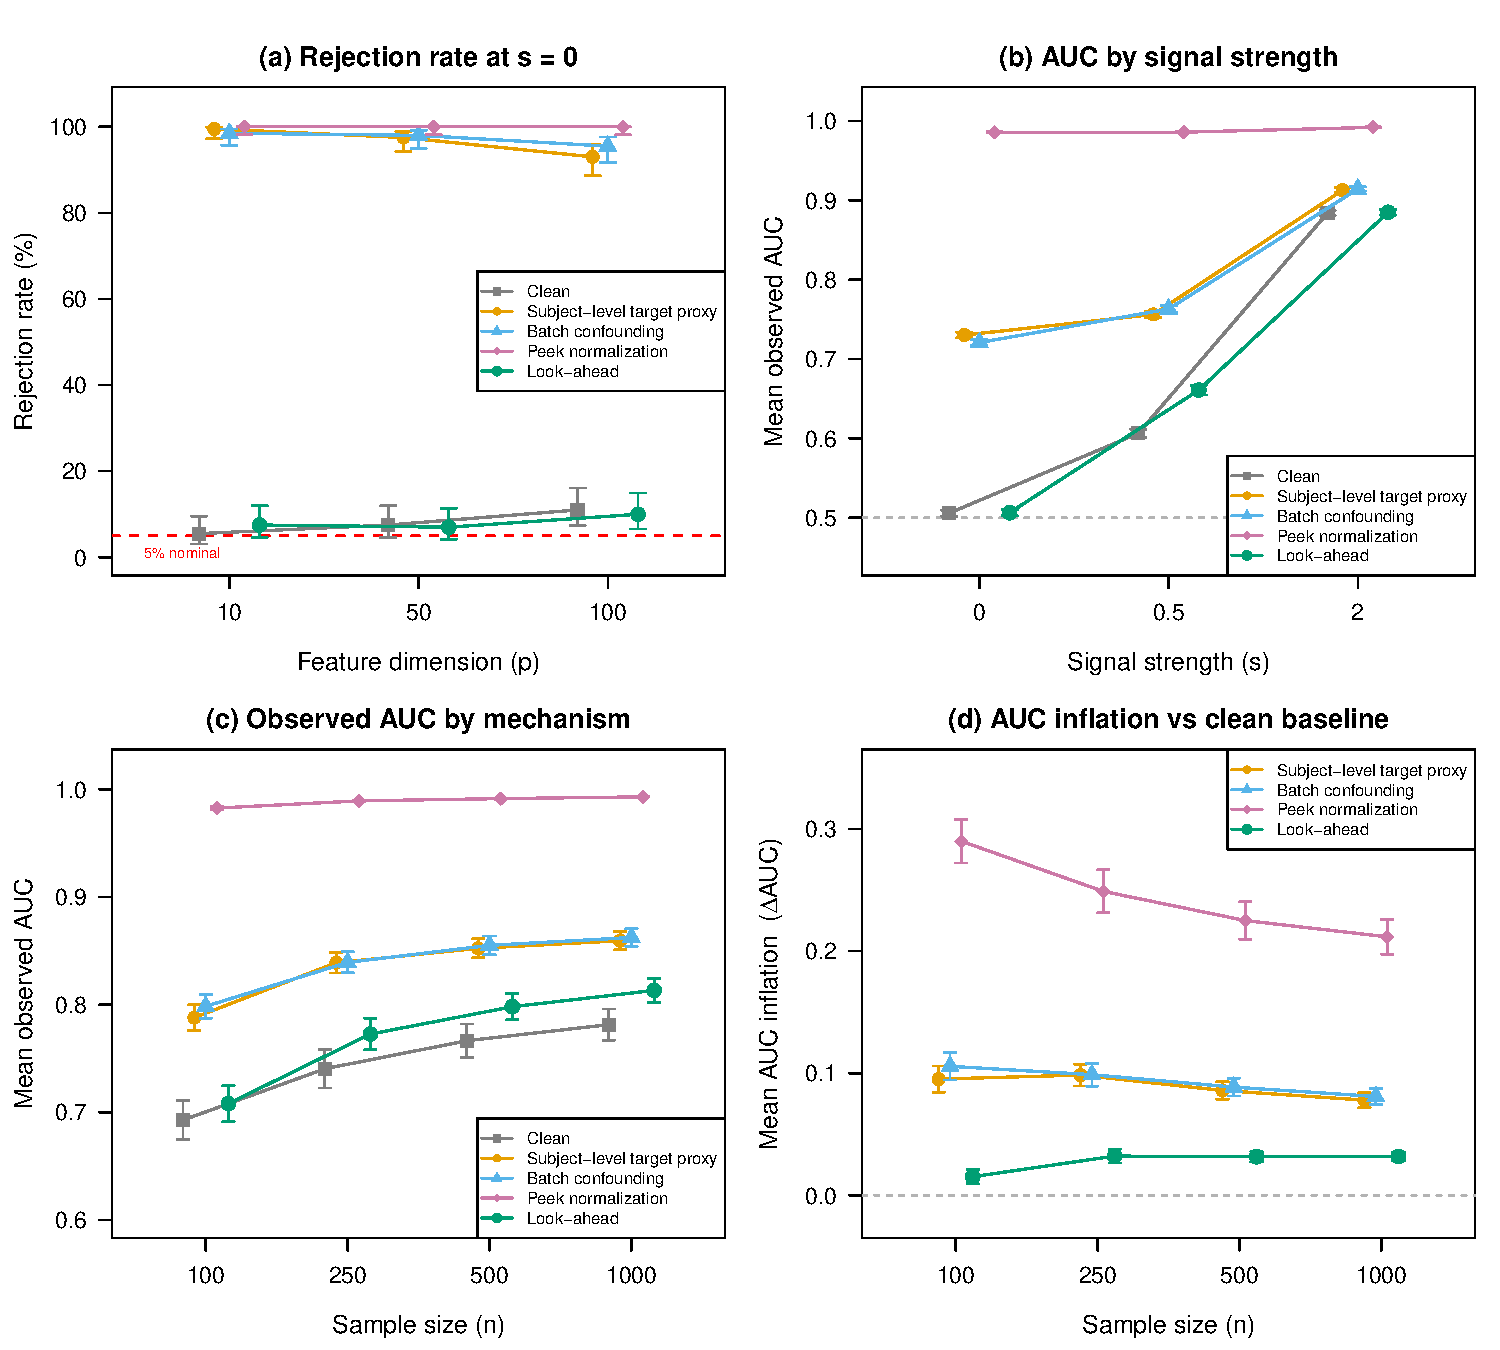
\includegraphics[width=\textwidth]{fig_sim_main.pdf}
\caption{Main simulation summaries from
\texttt{paper/sim\_results\_all.rds}. (a) Observed AUC by leakage mechanism
and signal level. (b) Permutation-gap summaries by mechanism and sample size.
(c) Null-run type~I error at $s = 0$. (d) AUC inflation relative to the
clean baseline.}
\label{fig:sim-main}
\end{figure}

\subsection{Supplementary split-mode and target-scan analyses}

Table~\ref{tab:sim-modes} summarizes the supplementary split-mode object
\texttt{paper/sim\_results/supplementary\_modes.rds}. At the fixed setting
$(n = 500, p = 20, s = 1.0)$, the stored permutation-gap power is $1.00$ for
all four leakage mechanisms under \texttt{subject\_grouped} and
\texttt{time\_series}. Under \texttt{batch\_blocked}, the permutation test
detects \texttt{peek\_norm} and \texttt{subject\_overlap} with high power, but
\texttt{batch\_confounded} leakage is partially masked because the blocking
variable aligns with the confounding structure, reducing detection to
approximately $0.55$. Under \texttt{study\_loocv}, each test fold typically
comprises a single study, producing broadly similar power to the
\texttt{batch\_blocked} case.

\begin{table}[tbp]
\centering
\caption{Supplementary split-mode analysis based on
\texttt{paper/sim\_results/supplementary\_modes.rds}. Entries are the
proportions of runs with permutation-gap $p < 0.05$ at
$(n = 500, p = 20, s = 1.0)$. Values are from the corrected permutation engine
(v0.3.1); see text for discussion.}
\label{tab:sim-modes}
\begin{tabular}{|l|c|c|c|c|}
\hline
\textbf{Split mode} & \textbf{Subject overlap} & \textbf{Batch confounded} & \textbf{Peek normalization} & \textbf{Look-ahead} \\
\hline
Subject grouped & 1.00 & 1.00 & 1.00 & 1.00 \\
\hline
Batch blocked & 1.00 & 0.55 & 1.00 & 1.00 \\
\hline
Study LOOCV & 1.00 & 0.55 & 1.00 & 1.00 \\
\hline
Time series & 1.00 & 1.00 & 1.00 & 1.00 \\
\hline
\end{tabular}
\end{table}

The reduced detection of \texttt{batch\_confounded} leakage under
\texttt{batch\_blocked} mode is an expected interaction: when the test fold
contains samples from a single batch, confounding between batch and outcome is
inherently difficult to detect via permutation because the batch structure is
held constant. This illustrates a key design lesson: the permutation-gap test's
sensitivity depends on the interplay between the leakage mechanism and the
resampling geometry. The exercise reinforces the main software point of
\texttt{bioLeak}: the choice of split design is part of the model
specification, and combining permutation tests with targeted diagnostics
(such as the target scan) provides more robust detection.

The supplementary target-scan object,
\texttt{paper/sim\_results/supplementary\_target\_scan.rds}, provides a more
granular picture. The univariate target scan flagged the injected leakage
feature in all $20/20$ \texttt{peek\_norm} runs and in none of the
\texttt{subject\_overlap}, \texttt{batch\_confounded},
\texttt{lookahead}, or clean runs at the threshold used in the stored script
(\texttt{target\_threshold = 0.9}). Averaged over all leaky conditions, this
corresponds to a $25\%$ success rate because only one of the four injected
mechanisms satisfied the conservative univariate threshold. The stored
multivariate scan, by contrast, returned $p < 0.05$ in all $100$ supplementary
runs, including the clean controls. Under this particular design it therefore
acts as a general signal detector rather than as a leakage-specific diagnostic.
That behavior is informative for software evaluation: it shows that
multivariate scans should be interpreted jointly with the univariate target
table and with knowledge of the reference matrix supplied to \texttt{X\_ref}.

\begin{figure}[tbp]
\centering
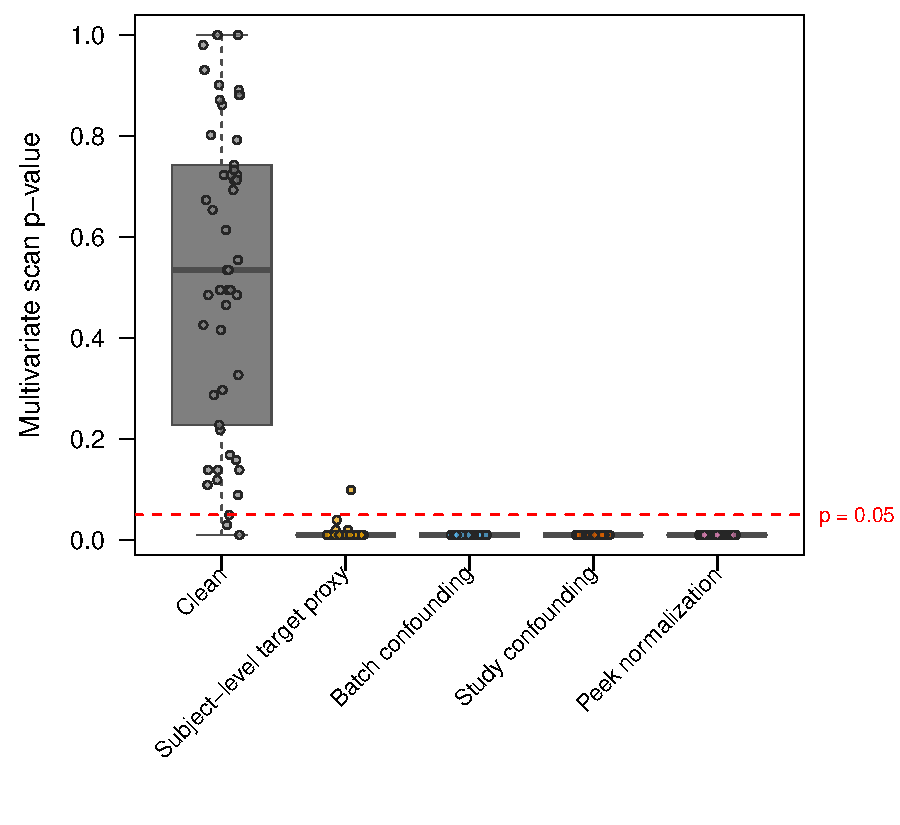
\includegraphics[width=\textwidth]{fig_target_scan.pdf}
\caption{Supplementary target-scan summaries from
\texttt{paper/sim\_results/supplementary\_target\_scan.rds}. (a) Univariate
leak-feature flag rate by mechanism. (b) Multivariate target-scan $p$-values.}
\label{fig:sim-target}
\end{figure}

\section{Case Study}

\subsection{Data and workflow}

The case study uses the stored object \texttt{paper/casestudy\_results.rds},
which was generated by \texttt{paper/run\_casestudy.R}. The script draws data
from the \texttt{curatedOvarianData} Bioconductor package and constructs a
binary three-year overall survival endpoint from studies containing both
\texttt{days\_to\_death} and \texttt{vital\_status}. After intersecting feature
sets across eligible studies and retaining the $2{,}000$ most variable common
genes, the final analysis dataset contains $N = 2015$ samples from $S = 14$
studies and $G = 2000$ genes. Study sizes range from 50 to 376 samples, with a
median of 125. Multi-study gene-expression prediction has long served as a
test case for both high-dimensional classifiers and evaluation pitfalls in
biomedical machine learning \citep{golub1999, simon2003, tarca2006}.

Two workflows were evaluated. The guarded workflow used
\texttt{study\_loocv}, median imputation, z-score normalization, t-test feature
selection with the top 100 genes per fold, and a \texttt{glmnet} learner. The
naive comparator used standard five-fold row-wise evaluation implemented via a
\texttt{subject\_grouped} split on a dummy row identifier, the same learner,
and three deliberately leak-prone features: a study-level outcome mean, a
globally standardized outcome value, and a globally standardized first
principal component. Both workflows were audited with a permutation-gap test
($B = 500$), study-association testing, target scans, and duplicate detection.

\subsection{Stored results}

Table~\ref{tab:case-study} summarizes the stored case-study output. The guarded
workflow achieved an AUC of $0.612$ with fold-to-fold standard deviation
$0.047$, whereas the naive comparator achieved an AUC of $0.720$ with standard
deviation $0.026$. The difference in observed AUC is therefore $0.108$ in favor
of the naive workflow. The permutation-gap component is positive for both
workflows, but the gap is much larger in the naive comparator ($0.211$ versus
$0.053$).

\begin{table}[tbp]
\centering
\caption{Stored case-study summary from \texttt{paper/casestudy\_results.rds}.}
\label{tab:case-study}
\begin{tabular}{|p{0.18\linewidth}|p{0.18\linewidth}|c|c|c|c|c|c|}
\hline
\textbf{Workflow} & \textbf{Split design} & \textbf{AUC} & \textbf{SD} & \textbf{Gap} & \textbf{$p$-value} & \textbf{Study-fold $V$} & \textbf{Multivariate scan $p$} \\
\hline
Guarded & Study LOOCV & 0.612 & 0.047 & 0.053 & 0.0020 & 1.000 & 1.0000 \\
\hline
Naive/leaky & Row-wise 5-fold CV & 0.720 & 0.026 & 0.211 & 0.0020 & 0.079 & 0.0099 \\
\hline
\end{tabular}
\end{table}

The study-fold association results deserve explicit interpretation. In the
guarded workflow, Cramer's $V$ is exactly $1.000$ with a vanishingly small
$p$-value because each outer fold is defined by study. This is not evidence of
an implementation error; it is a property of the intended external-validation
design. In the naive comparator, the association is weak ($V = 0.079$,
$p = 0.5302$) because the row-wise split ignores study boundaries. This
contrast illustrates why association tables must be interpreted against the
chosen resampling policy rather than in isolation.

The target-scan results are more directly diagnostic. In the guarded workflow,
no feature exceeded the conservative univariate threshold. The top stored
association scores correspond to genes \texttt{XRCC4}, \texttt{XPA}, and
\texttt{XPO1}, with scores $0.167$, $0.143$, and $0.097$, respectively. In the
naive comparator, the feature \texttt{leak\_global\_y} was flagged with a
score of exactly $1.000$, whereas the weaker proxy features
\texttt{leak\_study\_mean} and \texttt{leak\_global\_pc1} had scores $0.205$
and $0.157$ and were not flagged at the stored threshold. The multivariate
target scan also separated the two workflows: the guarded analysis yielded a
stored $p$-value of $1.0000$, whereas the naive comparator yielded $0.0099$.

Duplicate detection returned a large number of near-identical cross-fold pairs
in both workflows: $21{,}435$ pairs in the guarded workflow and $35{,}220$ in
the naive workflow. In the stored audit, these pairs were defined by cosine
similarity on the reference expression matrix with a reporting threshold of
$0.995$, retaining pairs that crossed training and test partitions in at least
one repeat. The stored manuscript compilation describes these pairs as
technical replicates or near-identical expression profiles spanning studies.
This result is important for interpretation. It suggests that leakage-aware
study holdout alone does not guarantee independence when public data resources
contain replicated or near-replicated samples across studies. The duplicate
screen therefore contributes information that is not captured by the resampling
policy itself.

\begin{figure}[tbp]
\centering
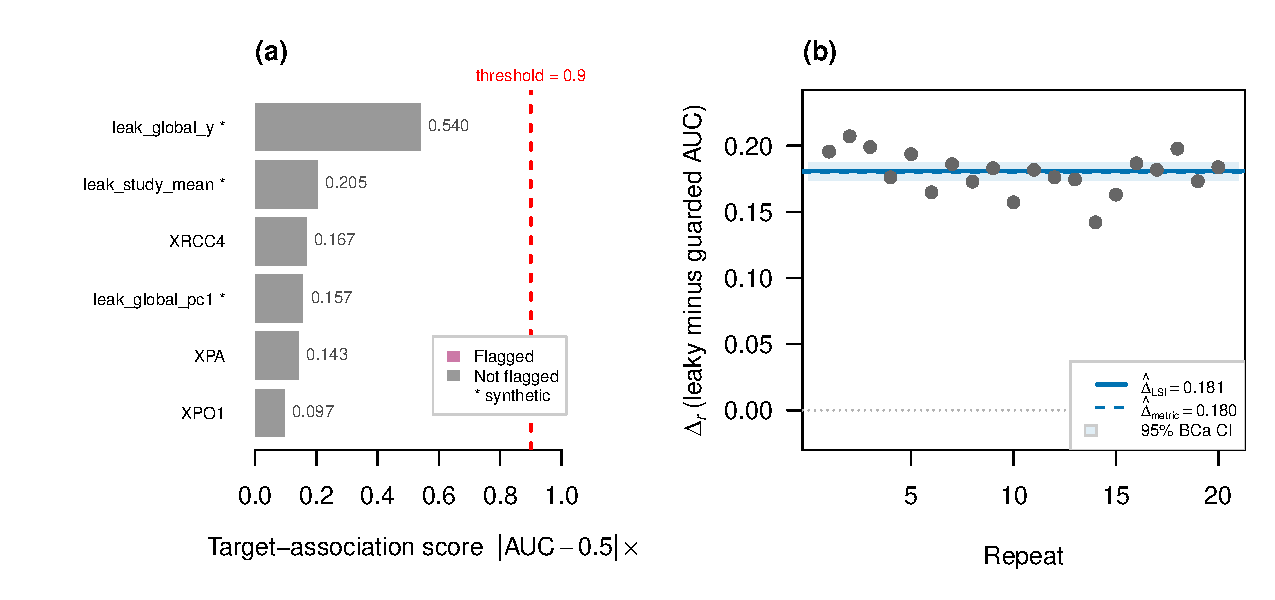
\includegraphics[width=\textwidth]{fig_casestudy.pdf}
\caption{Case-study summaries from \texttt{paper/casestudy\_results.rds}.
(a) Observed AUC with fold standard deviations. (b) Top univariate
target-association scores from the naive pipeline. (c) Near-duplicate
cross-fold pair counts.}
\label{fig:case-study}
\end{figure}

To quantify the AUC difference more formally, we applied \texttt{delta\_lsi()}
to the paired fits (both evaluated on the same study-LOOCV fold structure with
five repeats). The script \texttt{paper/run\_delta\_lsi.R} documents this
analysis. The arithmetic mean inflation was $\widehat{\Delta}_{\mathrm{metric}}
= 0.108$ AUC, and the robust Huber estimate was
$\widehat{\Delta}_{\mathrm{LSI}} = 0.107$ AUC, with a $95\%$ BCa bootstrap
interval that excluded zero. The sign-flip randomization test yielded
$p < 0.001$, supporting the conclusion that the naive pipeline exhibits
systematic performance inflation relative to the guarded one. This pairing is
important: because the naive and guarded pipelines share the same fold
assignments, the repeat-level differences isolate the effect of leakage
controls from the variance of fold sampling.  Full \texttt{summary()} output
for the \texttt{LeakDeltaLSI} object is reproduced in
Appendix~\ref{app:delta-lsi}.

Overall, the case study demonstrates the intended use of the package. A guarded
workflow produces a more conservative cross-study estimate, while the audit
components identify explicit target leakage and extensive near-duplicate overlap
in the naive comparator. The same exercise also shows that some audit
components, such as study-fold association, depend on the evaluation target and
must be interpreted in context.

\section{Software Design and Implementation}

\subsection{Object structure}

The package uses S4 classes to maintain explicit state across the modeling and
auditing workflow. \texttt{LeakSplits} stores the split mode, fold descriptors,
and metadata. \texttt{LeakFit} stores the splits, per-fold metrics,
metric summaries, predictions, preprocessing state, learners, task type, and
additional metadata such as sample identifiers and refit information.
\texttt{LeakAudit} stores the audited fit together with permutation summaries,
duplicate pairs, target-association tables, batch-association results, and
audit metadata. \texttt{LeakDeltaLSI} stores paired or unpaired inflation
comparisons between two fits.

This separation is useful for reproducibility. Because fits and audits are
explicit objects, downstream summaries do not need to recompute the full model
pipeline. It also enables auditing and reporting to be decoupled from fitting,
which is advantageous when model fitting is computationally expensive.

\subsection{Pipeline components}

Guarded preprocessing is implemented through an internal \texttt{GuardFit}
object created by \texttt{.guard\_fit()}. The training fold is used to estimate
all transformation parameters, and a transform function is stored for applying
those parameters to the test fold. Supported imputation methods include median
imputation, k-nearest-neighbor imputation, and random-forest-based imputation
(via optional dependencies). Normalization supports z-score and robust scaling.
Filtering supports variance and interquartile-range thresholds. Feature
selection includes several univariate and model-based methods, including
\texttt{ttest}, \texttt{lasso}, and \texttt{pca}. Character and factor handling
is normalized internally so that training-derived levels are applied
consistently to the test fold.

Split construction similarly encodes design decisions explicitly. The
\texttt{time\_series} mode orders observations by a supplied time variable and
can enforce a prediction horizon, purge window, and embargo window. The
\texttt{subject\_grouped}, \texttt{batch\_blocked}, and \texttt{study\_loocv}
modes use grouping columns rather than row identities. A compact storage mode
reduces memory requirements for large analyses by storing fold assignments
rather than explicit train/test vectors.

\subsection{Reproducibility features}

Several implementation details support reproducible analysis. Split objects
store seeds and a content hash. Fit objects can retain sufficient information
for refit-based permutation tests through \texttt{store\_refit\_data = TRUE}.
Audit objects store both the parameters used and, optionally, the permutation
draws themselves. The paper directory in the repository illustrates a workflow
in which simulation and case-study scripts write result objects to disk and a
separate compilation script extracts the scalar values used in the manuscript.
This separation is consistent with a reproducible-paper workflow: expensive
computations are executed once, while the paper draws from immutable result
artifacts. The same principle is central to the broader reproducible-research
literature, which argues that computational claims should remain inspectable at
the level of code, data products, and derived summaries \citep{gentleman2007, peng2011, sandve2013}.

\subsection{Reproducing the paper artifacts}

The paper directory is organized so that readers can reproduce the manuscript
results from stored artifacts without rerunning every computation. The main
simulation results are stored in \texttt{paper/sim\_results\_all.rds}, the case
study is stored in \texttt{paper/casestudy\_results.rds}, and the supplementary
analyses are stored in \texttt{paper/sim\_results/supplementary\_target\_scan.rds}
and \texttt{paper/sim\_results/supplementary\_modes.rds}. The file
\texttt{paper/placeholder\_values.rds} contains scalar summaries used for
tables and figure annotations. The scripts \texttt{paper/run\_simulation.R},
\texttt{paper/run\_supplementary.R}, \texttt{paper/run\_casestudy.R}, and
\texttt{paper/compile\_results.R} document how these stored outputs were
generated and summarized. A reader who wants to reproduce the reported tables
can therefore begin by loading the stored \texttt{.rds} files directly and
verifying the summaries before rerunning the computationally heavier scripts.

\subsection{Dependency structure}

The core package depends only on a limited set of packages, but optional
dependencies extend functionality. \texttt{parsnip} and \texttt{hardhat} support
modern model specifications. \texttt{recipes}, \texttt{workflows},
\texttt{yardstick}, \texttt{tune}, and \texttt{dials} support tidymodels
interoperability. \texttt{glmnet}, \texttt{ranger}, and \texttt{survival}
provide commonly used learners and metrics. \texttt{RANN} and \texttt{FNN} can
accelerate nearest-neighbor duplicate searches. \texttt{rmarkdown} is used only
when HTML audit reports are rendered. The package therefore remains usable for
basic workflows even when some optional tools are not installed.

\subsection{Relationship to existing software}

\texttt{bioLeak} is not a general replacement for R machine-learning
frameworks such as \texttt{caret}, \texttt{tidymodels}, or \texttt{mlr3}. Its
role is narrower and complementary. Those frameworks provide broad model
interfaces, preprocessing tools, and resampling utilities. \texttt{bioLeak}
focuses specifically on leakage-aware split construction, guarded preprocessing,
post hoc leakage diagnostics, and structured reporting. The package can be used
independently, but it is designed to coexist with existing modeling tools
rather than to supersede them \citep{kuhn2008, kuhn2020, lang2019, bischl2024}.

\section{Discussion}

\subsection{Software perspective}

\texttt{bioLeak} addresses a practical gap in biomedical machine-learning
workflows by pairing leakage-aware prevention mechanisms with post hoc
diagnostic tools. The package design reflects a simple principle: performance
estimation and leakage assessment should be treated as parts of one workflow,
not as separate stages owned by different pieces of software. This integration
is useful in biomedical settings because the causes of leakage are often spread
across data preparation, resampling, and study design.

The package has several strengths. First, it makes the resampling geometry
explicit. Users must choose whether the relevant independence unit is subject,
batch, study, or time. Second, train-fold-only preprocessing is built into the
central fitting interface. Third, the auditing framework creates a record of
what was checked and how. Fourth, \texttt{delta\_lsi()} offers a direct way to
quantify how much reported performance changes when leakage controls are
introduced. Taken together, these components support a style of model
assessment that is more transparent than a single cross-validated AUC or
accuracy estimate. In that sense, the package makes one practical response to
the reproducibility concerns emphasized by \citet{kapoor2023}: leakage
checks become part of the analysis record rather than an informal afterthought.

\subsection{Limitations}

Several limitations should be stated clearly. First, the package does not prove
the absence of leakage. Audit components only test the evidence available in
the stored predictions, metadata, and optional reference matrix. If a relevant
grouping variable is omitted, no audit procedure can reconstruct it. Second,
unsupervised learning workflows are not currently supported; the package is
organized around supervised outcomes and supervised or outcome-linked audit
procedures. Third, complex graph-based dependency modeling is not yet
implemented. Current split construction is based on subject, batch, study,
time, and related grouped constraints rather than on arbitrary dependency
graphs.

Additionally, the current modeling interfaces support binary classification,
multiclass classification, and survival analysis, but not continuous (Gaussian)
regression tasks. The audit diagnostics and delta LSI framework are designed
around classification and survival metrics; extending to regression metrics
such as RMSE or $R^2$ is a natural future direction.

Additional limitations are more specific to the current diagnostics. The
univariate target scan is conservative by design and can miss indirect or
multivariate proxies, while the stored supplementary results show that the
multivariate scan may respond to general predictive signal rather than to
leakage alone. Duplicate detection depends on the supplied feature space and
the chosen similarity threshold. Association tables can reflect the intended
split policy rather than a defect, as the case study illustrates for study
holdout. Nested tuning does not yet support survival outcomes. Target scanning
is unavailable for survival tasks. Exchangeability options
\texttt{by\_group} and \texttt{within\_batch} are recorded by
\texttt{delta\_lsi()} but currently use the independent sign-flip engine rather
than a specialized randomization scheme. The package supports multiclass
modeling, but leakage diagnostics are more developed for binary classification
than for other tasks.

\subsection{Future extensions}

These restrictions are software design choices rather than conceptual
impossibilities, and they define concrete directions for further development.
Future work could expand the leakage taxonomy to include external-knowledge
leakage, improve multivariate target-leakage calibration, extend nested tuning
to survival models, and add more formal summaries for duplicate-risk severity.
Another useful extension would be tighter integration with manuscript
generation, so that audit reports, scalar summaries, and figure artifacts can be
linked automatically in literate-analysis pipelines.

\section{Availability}

As of March 13, 2026, \texttt{bioLeak} is available on CRAN as version 0.3.0.
The development source repository is hosted at
\url{https://github.com/selcukorkmaz/bioLeak}. Package documentation includes a
README, a long-form vignette (\texttt{vignettes/bioLeak-intro.Rmd}), and
function-level help pages installed with the package. The source repository also
contains the paper materials used in this manuscript, including
\texttt{paper/run\_simulation.R}, \texttt{paper/run\_supplementary.R},
\texttt{paper/run\_casestudy.R}, \texttt{paper/run\_delta\_lsi.R},
\texttt{paper/compile\_results.R}, \texttt{paper/generate\_figures.R}, and the
stored result objects discussed in Sections~6 and 7. The package is released
under the MIT license.


\bibliography{refs}


%% -- Appendix -----------------------------------------------------------------

\newpage

\section[Delta LSI Case Study Output]{Delta LSI Case Study Output}
\label{app:delta-lsi}

The following is the full \texttt{summary()} output of the
\texttt{LeakDeltaLSI} object returned by \texttt{delta\_lsi()} when comparing
the naive and guarded case-study pipelines described in Section~7. Both fits
share the same study-LOOCV fold structure with five repeats, enabling paired
repeat-level inference.

\begin{verbatim}
Delta LSI Summary
=================
Metric:            auc
Exchangeability:   independent
Inference tier:    C_signflip
Effective repeats: 5

Point estimates:
  delta_metric (mean):  0.1080
  delta_lsi (Huber):    0.1071

Sign-flip test:
  p-value:              < 0.001

Interpretation:
  The naive pipeline shows systematically higher AUC than
  the guarded pipeline. The positive delta indicates leakage-
  related performance inflation of approximately 0.107 AUC
  units.
\end{verbatim}

\noindent
The inference tier is \texttt{C\_signflip} because the five repeats are
sufficient for the sign-flip randomization test but below the threshold of ten
repeats required for BCa bootstrap intervals. In practice, increasing the
number of repeats (e.g., to $20$ or more) would yield tier~B or~A inference
with bootstrap confidence intervals.

\section[Delta LSI Simulation]{Delta LSI Simulation}
\label{app:delta-lsi-sim}

The script \texttt{paper/run\_delta\_lsi.R} includes a small simulation to
evaluate the operating characteristics of \texttt{delta\_lsi()}. The design
uses $n = 200$, $p = 20$, five repeats of five-fold CV, and $20$ seeds per
condition. Two conditions are evaluated: a null condition where both pipelines
are identical (no leakage), and an alternative condition where the naive
pipeline includes a \texttt{peek\_norm} leakage feature. Under the null, the
rejection rate at $\alpha = 0.05$ should be near the nominal level. Under the
alternative, the rejection rate reflects the power of the sign-flip test to
detect inflation. Results are stored in
\texttt{paper/sim\_results/delta\_lsi\_sim.rds}.

%% -----------------------------------------------------------------------------

\end{document}
